\documentclass[UTF8]{beamer}
\usepackage{graphicx}
\usepackage{mathrsfs}

% bottom info
\setbeamertemplate{footline}{
	\leavevmode
	\hbox{
		\begin{beamercolorbox}[wd=.25\paperwidth,ht=2.25ex,dp=1ex,center]{author in head/foot}
			\usebeamerfont{author in head/foot}\insertshortauthor
		\end{beamercolorbox}
		\begin{beamercolorbox}[wd=.5\paperwidth,ht=2.25ex,dp=1ex,center]{title in head/foot}
			\usebeamerfont{title in head/foot}\insertshorttitle
		\end{beamercolorbox}
		\begin{beamercolorbox}[wd=.2\paperwidth,ht=2.25ex,dp=1ex,right]{date in head/foot}
			\usebeamerfont{date in head/foot}\insertshortdate{}\hspace*{2em}
			\insertframenumber{} / \inserttotalframenumber\hspace*{2ex}
	\end{beamercolorbox}}
	\vskip0pt
}

% highlight Section
\AtBeginSection[]
{
  \begin{frame}
    \frametitle{Catalogs}
    \tableofcontents[currentsection]
  \end{frame}
}

% superscript reference
\makeatletter
\def\@cite#1#2{\textsuperscript{[{#1\if@tempswa , #2\fi}]}}
\makeatother

%---------text---------%

\title[Contrastive Multi-View Representation Learning on Graphs]{Contrastive Multi-View Representation Learning on Graphs\cite{hassani2020contrastive}}

\author[reporter: Xingyu Ji]{reporter: Xingyu Ji}

\institute[] {
	\textit{paper author: Kaveh Hassani, Amir Hosein Khasahmadi}  \\
	\medskip
	\textit{Proceedings of the 37 th International Conference on Machine
    Learning, Vienna, Austria, PMLR 108, 2020. Copyright 2020 by
    the author(s).}
    \date{today}
}

\begin{document}

    \begin{frame}
        \titlepage
    \end{frame}

    \section{Introduction}

    \subsubsection{Process}

    \begin{frame}
        \frametitle{Process}
        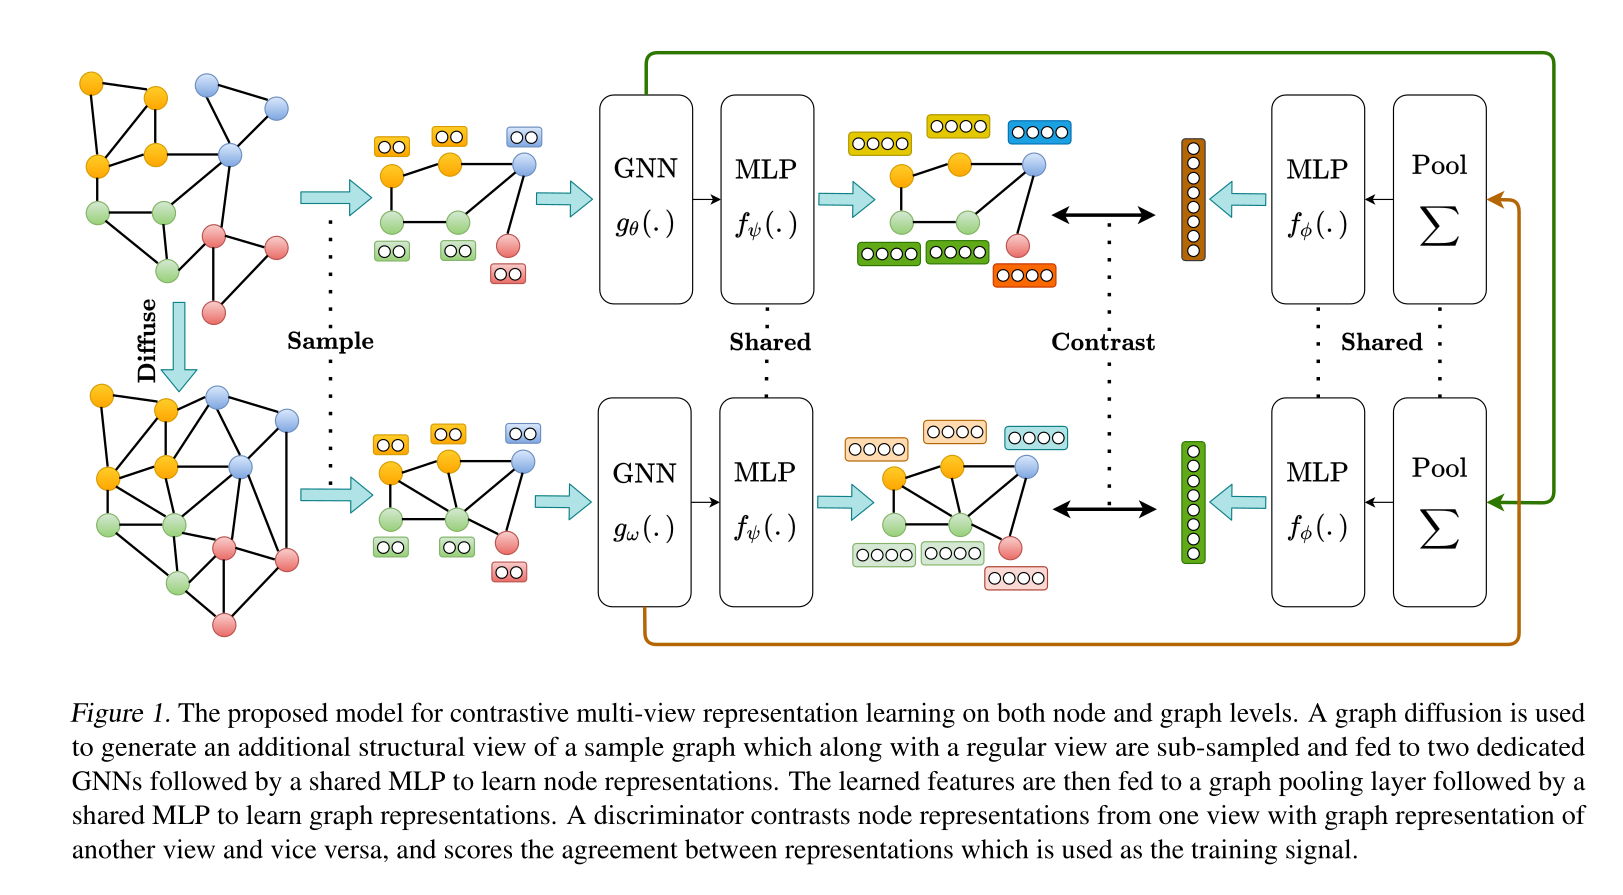
\includegraphics[width=\linewidth]{./images/process.png}
    \end{frame}

    \subsubsection{Graph Diffusion Network}

    \begin{frame}
        \frametitle{Graph Diffusion Network}

        \begin{enumerate}
            \item PPR
            
            GCN appearence: GCN converges to the random walk’s limit distribution as the number of layers increases.
        
            $\rightarrow$ GCN problem: Only relevant to the full graph, not to the root node
            \vspace{.5cm}

            $\Rightarrow$ Increasing the probability of jumping back to the root node in PageRank \cite{gasteiger2018predict} ( Personalized PageRank, PPR )

            \item heat
            
            A very mathematical approach to localized diffusion

        \end{enumerate}

    \end{frame}

    \begin{frame}
        \frametitle{Graph Diffusion Network}
    
        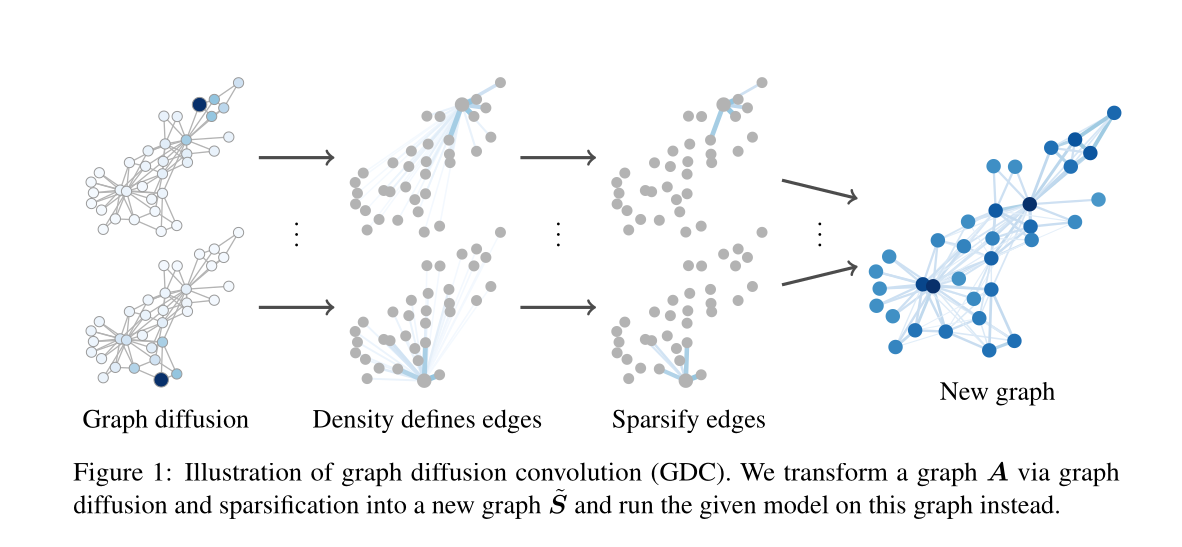
\includegraphics[width=\linewidth]{./images/diffusion.png}
    
    \end{frame}
    
    \subsubsection{InfoMax}

    \begin{frame}
        \frametitle{InfoMax}

        Mutual information:

        \begin{equation*}
            \begin{aligned}
                I(X;Y) &= \int_{Y}\int_{X}p(x,y)log\frac{p(x,y)}{p(x)p(y)}dxdy  \\
                &= \int_{Y}\int_{X}p(y|x)p(x)log\frac{p(y|x)}{p(y)}dxdy
            \end{aligned}
        \end{equation*}

        max the $I(X;Y)\ \Rightarrow$ max $\frac{p(y|x)}{p(y)}$
        \vspace{.5cm}

        $\Rightarrow$ max $KL(p(x,y)||p(x)p(y))$

    \end{frame}

    \section{Method}

    \subsubsection{Augmentations}

    \begin{frame}
        \frametitle{Augmentations}
        we consider 2 types of augmentations on graphs:
        \begin{enumerate}
            \item feature-space augmentations (operating on init node features) (e.g. masking or adding Gaussian noise)
            \item structure-space augmentations and corruptings (operating on graph structure) (e.g. adding or removing connectivities, sub-sampling, generating global views using shortest dst or generating diffusion matrices)
        \end{enumerate}
        \vspace{.5cm}

        former aug. problem:
        \begin{enumerate}
            \item benchmarks do not carry initial node features
            \item degrades the performance
        \end{enumerate}
        \vspace{.5cm}
        
        $\rightarrow$ using aug.2

        shiyande aug.2-generating diffusion matrices the best.
        \vspace{.5cm}

        we treating the two matrices (ori \& diffusion) as two congruent views of the same graph's structure

    \end{frame}

    \begin{frame}
        \frametitle{Augmentations}

        diffusion is formulated as Eq.1

        \begin{equation*}
            S = \sum_{k=0}^\infty \Theta_kT^k, \quad S\in\mathbb{R}^{n\times n}  \tag{1}
        \end{equation*}

        where $T$ is the generalized transition matrix.

        \begin{equation*}
            \begin{aligned}
            & \text{adjacency matrix: } A\in\mathbb{R}^{n\times n}  \\
            & \text{diagonal degree matrix: } D\in\mathbb{R}^{n\times n}  \\
            \end{aligned}  
        \end{equation*}
        \begin{equation*}
            T = AD^{-1}
        \end{equation*}

        So $T$ is normalized the adjacency matrix ( $D^{-1}$ is the reciprocal of the \textbf{value} of $D$).
        \vspace{.5cm}

    \end{frame}

    \begin{frame}
        \frametitle{Augmentations \cite{gasteiger2019diffusion}}
    
        In Eq.1, $\Theta$ is the weighting coefficient which determines the ratio of global-local information.

        \begin{equation*}
            \Theta \text{ s.t. } \sum_{k=0}^\infty\theta_k = 1, \quad \theta_k \in [0,1]
        \end{equation*}

        And for $\theta_k$ ,

        \begin{equation*}
            \begin{aligned}
                \theta_k^{heat} &= \frac{e^{-t}t^k}{k!}  \\
                \theta_k^{PPR} &= \alpha(1-\alpha)^k
            \end{aligned}
        \end{equation*}

        Where $\alpha$ denotes teleport probability in a random walk, and $t$ is diffusion times.

        So the heat kernel \& Personalized PageRank (PPR) is:

        \begin{equation*}
            \begin{aligned}
            S^{heat} &= \exp(tAD^{-1}-t)  \\
            S^{PPR} &= \alpha[I_n - (1-\alpha)D^{-\frac{1}{2}}AD^{-\frac{1}{2}}]^{-1}
            \end{aligned}
        \end{equation*}
    
    \end{frame}

    \subsubsection{Encoder}

    \begin{frame}
        \frametitle{Encoder}
        using GCN method
    
        input: \(A\ S\ X\ \Theta\)
        \begin{enumerate}
            \item \(A\) : ori adj mat \(\in\mathbb{R}^{n\times n}\)
            \item \(S\) : diffusion mat (adj + ind) \(\in\mathbb{R}^{n\times n}\)
            \item \(X\) : init node features \(\in\mathbb{R}^{n\times d_x}\)
            \item \(\Theta\) : the network parameters \(\in\mathbb{R}^{d_x\times d_h}\)
                \begin{itemize}
                    \item \(d_x\) : dim of init node features
                    \item \(d_h\) : dim of output features
                \end{itemize}
        \end{enumerate}
        
    \end{frame}
    
    \begin{frame}
        \frametitle{Encoder}

        GCN layer: \(\sigma(\tilde{A}X\Theta)\) and \(\sigma(SX\Theta)\)
        \vspace{.5cm}
        
        where \(\tilde{A} = \tilde{D}^{-\frac{1}{2}}\hat{A}\tilde{D}^{-\frac{1}{2}}\), \(\tilde{D}\) is the degree mat of \(\hat{A} = A+I_N\)
        
        \begin{equation*}
            g_\theta(.)/g_\omega(.) : \mathbb{R}^{n\times n}[\cdot\mathbb{R}^{n\times d_x}\cdot\mathbb{R}^{d_x\times d_h}] \rightarrow \mathbb{R}^{n\times d_h}
        \end{equation*}
        
        \(\theta\) repre. original mat parameters

        \(\omega\) repre. diffusion mat parameters  
        \vspace{.5cm}
        
        And then 2 hidden layer MLP \(f_\psi(x) = \text{PReLU}(w_\psi^Tx)\)
        
        \begin{equation*}
            f_\psi(.) : \mathbb{R}^{n\times d_h} \rightarrow \mathbb{R}^{n\times d_h}
        \end{equation*}
        
        so we have the two set of node features of ori \& diffusion graph
        
        \begin{equation*}
            H^\alpha = f_\psi(g_\theta(.))
            H^\beta = f_\psi(g_\omega(.)) \in\mathbb{R}^{n\times d_h}
        \end{equation*}        
    
    \end{frame}

    \begin{frame}
        \frametitle{Encoder}

        then for each view, we use a readout function similar to JK-Net to aggregate the node repre.
        
        \begin{equation*}
            \vec{h_g} = \sigma(\Vert_{l=1}^L(\sum_{i=1}^n\vec{h_i^l})\cdot W)\in\mathbb{R}^{1\times d_h}  \tag{2}
        \end{equation*}
        
        where \(W\in\mathbb{R}^{(L\times d_h)\times d_h}\) is the network parameters.
        \vspace{.4cm}
        
        Eq.2 sum all nodes' repre. of a GCN layer (\(\rightarrow\mathbb{R}^{1\times d_h}\)) and concat all layers' res (\(\rightarrow\mathbb{R}^{L\times d_h}\)). and then \(\cdot W\) (\(\rightarrow\mathbb{R}^{1\times d_h}\))
        \vspace{.4cm}
        
        then 2 hidden layer MLP \(f_\phi(x) = \text{PReLU}(w_\phi^Tx)\)
        \vspace{.4cm}
        
        finally get the graph repre. \(\vec{h_g^\alpha}\ \vec{h_g^\beta}\) and node repre. \(H^\alpha\ H^\beta\)
        \vspace{.4cm}
        
        for every view: init node features $\stackrel{GCN1}{\rightarrow}$ \(\vec{h^1}\) $\stackrel{GCN2}{\rightarrow}$ ... $\stackrel{GCNL}{\rightarrow}$ \(\vec{h^L}\)
        
        $\Rightarrow$ \(\vec{h_g}\) \& \(H^{\cdot}\)        
    
    \end{frame}

    \subsubsection{Training}

    \begin{frame}
        \frametitle{Training}

        so we have the fuction $g_\cdot\ f_\cdot$ ,and $g_\cdot$ is GCN fuction, $f_\cdot$ is MLP function, and the parameters index are $\theta\ \omega\ \psi\ \phi$
        \vspace{.5cm}

        and we should learn the rich node and graph level repre. that are agnostic to down-stream tasks $\rightarrow$ max the Deep InfoMax of diff. view
        \vspace{.5cm}

        so our optimize function:

        \begin{equation*}
            max_{\theta\ \omega\ \psi\ \phi}\ \frac{1}{|\mathscr{G}|}\sum_{g\in\mathscr{G}}\{\frac{1}{|g|}\sum_{i=1}^{|g|}[MI(\vec{h_i^\alpha, h_g^\beta}) + MI(\vec{h_i^\beta, h_g^\alpha})]\}  \tag{3}
        \end{equation*}

        $g$ is the sub-sampled graph of one view and select the exact nodes and edges from the other view. And $|\mathscr{G}|$ is the number of sub-sampled graphs.
        \vspace{.5cm}

    \end{frame}

    \begin{frame}
        \frametitle{Training}

        $MI(.,.)$ takes in a node repre. from one view ( $\vec{h_i^\alpha}$ ) and a graph repre. from another view ( $\vec{h_g^\beta}$ ). Here we simply dot product between them

        \begin{equation*}
            MI(\vec{h_i^\alpha, h_g^\beta}) = \vec{h_i^\alpha}\cdot\vec{h_g^\beta}^T
        \end{equation*}

        ( $\mathbb{R}^{1\times d_h}\cdot\mathbb{R}^{d_h}\rightarrow\mathbb{R}$ )
    
    \end{frame}

    \section{Experimental Results}

    \subsection{Ablation Study}

    \begin{frame}
        \frametitle{Ablation Study}

        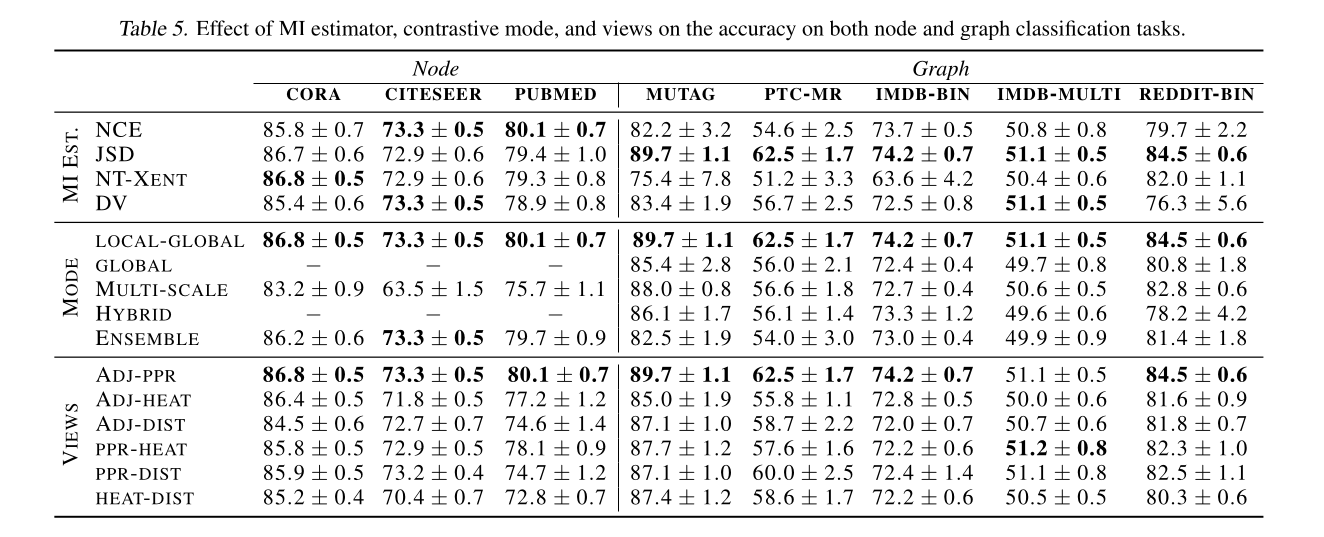
\includegraphics[width=\linewidth]{./images/ablation.png}

        
    
    \end{frame}

    \section{Refrence}

    \begin{thebibliography}{99}
        
        \bibitem{hassani2020contrastive}
        K.~Hassani and A.~H. Khasahmadi, ``Contrastive multi-view representation learning on graphs,'' in \emph{International conference on machine learning}.\hskip 1em plus 0.5em minus 0.4em\relax PMLR, 2020, pp. 4116--4126.

        \bibitem{gasteiger2018predict}
        J.~Gasteiger, A.~Bojchevski, and S.~G{\"u}nnemann, ``Predict then propagate: Graph neural networks meet personalized pagerank,'' \emph{arXiv preprint arXiv:1810.05997}, 2018.

        \bibitem{gasteiger2019diffusion}
        J.~Gasteiger, S.~Wei{\ss}enberger, and S.~G{\"u}nnemann, ``Diffusion improves graph learning,'' \emph{Advances in neural information processing systems}, vol.~32, 2019.

    \end{thebibliography}

\end{document}